\documentclass{replab}
\usepackage{lipsum}
\usepackage[shortlabels]{enumitem}

% --- Información del documento ---
\title{Taller - Semana 4}
\author{Diego Alejandro Heredia Franco}

% Nota: Si se desea incluir más de un autor en el documento, el archivo replab.cls, en la sección "Página de título de documento", contiene líneas de código comentadas pensadas para introducir los datos desde 1 hasta 4 autores. Sin embargo, debe escogerse solo una de las cuatro secciones de código y comentar las demás para mantener la consistencia del documento.

\date{23/24 de abril de 2025}
\subtitle={Física - Cinemática 1D/2D}
\email={\href{mailto:dherediaf@unal.edu.co}{\color{principaluno}\texttt{dherediaf@unal.edu.co}}}
\subject={Taller Fundamentos de Mecánica}

\setlength{\columnsep}{14pt}

% --- Archivo de bibliografía ---
\addbibresource{repbib.bib}

% --- Inicio del documento ---
\begin{document}
\setlength{\parindent}{0pt}
	
	\pagestyle{fancy}
	\unspacedoperators
	
% --- Título ---
	{\begin{tcolorbox}[colframe=white, colback=principaldos, arc=8pt]
		\begin{center}
			\maketitle
			%\rule{\textwidth}{0.2pt}
			%\medskip

			%\noindent\textit{Palabras Clave:} medidas directas e indirectas, análisis estadístico, incertidumbre, calibrador Vernier, balanza.
		\end{center}
	\end{tcolorbox}}
	\selectlanguage{spanish}

	Los ejercicios que aquí se presentan, a excepción de la primera tanda (i.e física y geometría), han sido tomados de \cite{lanaturaleza}, \cite{serway} y \cite{londono} en los capítulos relacionados con cinemática y movimiento 1D/2D.\\

{\begin{tcolorbox}[colframe=red!50!black, colback=red!5!white, arc=8pt]
	\textbf{Sugerencia:} En el libro \textit{Física para Ciencias e Ingeniería} (Serway) \cite{serway}, se presenta al final de cada capitulo un \textit{\textbf{resumen de los conceptos más importantes}}, así como un pequeño manuscrito con un \textit{\textbf{paso a paso general para resolver problemas}}. Se recomienda fuertemente al estudiante leer este instructivo para que pueda resolver los ejercicios de forma más organizada y eficiente.
\end{tcolorbox}}

% --- Cuerpo del reporte ---
	\section{Física y Geometría}

	\subsection{Ejercicio: Mínima Área Superficial}
	Demuestre que un cilindro recto con determinado volumen $V$ tiene un área superficial mínima cuando su altura $h$ es igual a su diámetro $d$. El kilogramos patrón se fabricó según este criterio para reducir al mínimo los errores debidos a la contaminación o corrosión de su superficie. 

	\subsection{Ejercicio: Altura de una Montaña}
	Cuando Galileo utilizó el telescopio para observar la luna, notó algunas manchas, siendo la más protuberante la identificada en la (Fig. \ref{fig:montana}) como $A$. Estas manchas Galileo las interpretó como la luz reflejándose en la cima de una montaña cuya base permanecía en la oscuridad. Si se toma la distancia $d$ como $1/10$ el radio lunar medio $R_M \approx 1740km$. Calcule la altura $h$ de la montaña y compárela con la del monte Everest.

	\begin{figure}[htbp]
		\centering
		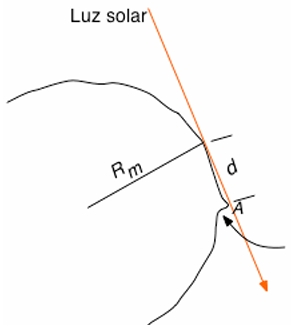
\includegraphics[width=.3\columnwidth]{imagenes/luna.jpeg}
		\caption{Dibujo esquemático de la luna.}
		\label{fig:montana}
	\end{figure}

	\subsection{Ejercicio: Rocío y su Espesor \textcolor{red}{*}}
	Se afirma que el espesor de la capa de rocío presente sobre la superficie de una hoja es de $1\mu g/cm^2$. Explique porque tiene sentido dar el espesor de la hoja en estas unidades $\mu g/cm^2$ y exprese dicho espesor en nanómetros. 

	\section{Desplazamiento, Velocidad y Aceleración}

	\subsection{Ejercicio: Pista de Carreras}
	Una pista de carreras es ovalada, con lados rectos de $3.0km$ y extremos circulares en ambos lados de $1.0km$ de radio cada uno (Fig. \ref{fig:pista}). Un automóvil la recorre en $7.0min$, en sentido de las manecillas del reloj. ¿Cuál es la velocidad media durante una vuelta completa? Suponiendo rapidez constante, ¿cuál es la velocidad instantánea en los puntos A y B? 

	\begin{figure}[htbp]
		\centering
		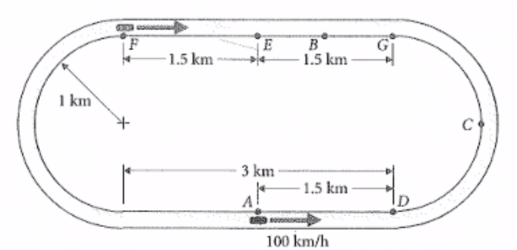
\includegraphics[width=.4\columnwidth]{imagenes/pista.png}
		\caption{Dibujo esquemático de la pista de carreras.}
		\label{fig:pista}
	\end{figure}

	\subsection{Ejercicio: Relación entre Velocidad y Aceleración \textcolor{red}{*}}
	Una partícula recorre la trayectoria indicada por la línea de puntos de la (Fig. \ref{fig:trayectoria}). Cuando se encuentra en el punto $A$ su velocidad aumenta. ¿Con cuál de los vectores que aparecen en ese punto se representa mejor esa aceleración? Explique por qué el que indicó es correcto y los demás son erróneos. 

	\begin{figure}[htbp]
		\centering
		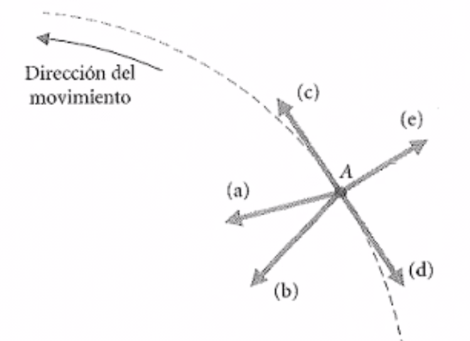
\includegraphics[width=.4\columnwidth]{imagenes/trayectoria.png}
		\caption{Dibujo esquemático de la trayectoria de la partícula.}
		\label{fig:trayectoria}
	\end{figure}

	\subsection{Ejercicio: Vector de Posición}
	El vector de posición de una partícula varía en el tiempo de acuerdo con la expresión $\vec{r} = (3.00\hat{i} - 6.00t^2\hat{j})m$. a) Encuentre expresiones para la velocidad y la aceleración de la partícula en función del tiempo. b) Determine la posición y velocidad de la partícula en $t = 1.00s$.  

	\section{Movimiento 1D}

	\subsection{Ejercicio: Canica sobre una Pista}
	Una niña rueda una canica sobre una pista con dobleces que mide $100cm$ de largo, como se muestra en la (Fig. \ref{fig:pista2}). Use x para representar la posición de la canica a lo largo de la pista. En las secciones horizontales de $x=0cm$ a $x=20cm$ y de $x=40cm$ a $x=60cm$, la canica se mueve a una rapidez constante. En las secciones de pendiente, la rapidez de la canica cambia de manera uniforme. En los lugares donde la pendiente cambia, la canica permanece en la pista y no experimenta cambios súbitos de rapidez. La niña da a la canica cierta rapidez inicial en $x=0cm$ y $t=0s$ y luego la observa rodar a $x=90cm$ donde regresa, y eventualmente regresa a $x=0cm$ con la misma rapidez inicial con la que al inicio la niña la liberó. Prepare graficas de $x$ en función de $t$, de $v_x$ en función de $t$ y de $a_x$ en función de $t$. 
	
	\begin{figure}[htbp]
		\centering
		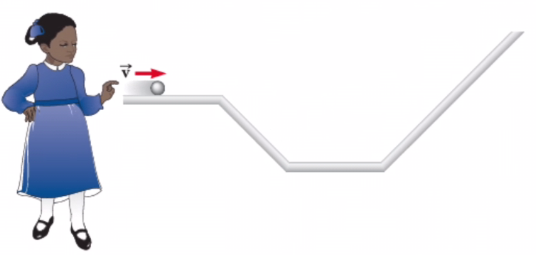
\includegraphics[width=.4\columnwidth]{imagenes/pista2.png}
		\caption{Dibujo esquemático de la pista para la canica.}
		\label{fig:pista2}
	\end{figure}

	\subsection{Ejercicio: Tiempo de Caída}
	Una bola se lanza directamente hacia arriba, con una rapidez inicial de $8.00m/s$, desde una altura de $30.0m$. ¿Después de qué intervalo de tiempo la bola golpea el suelo?
	
	\subsection{Ejercicio: Marcas de Derrape}
	El conductor de un automóvil aplica los frenos cuando ve un árbol que bloquea el camino. El automóvil frena uniformemente con una aceleración de $-5.60m/s^2$ durante $4.20s$, y hace marcas de derrape rectas de $62.4m$ de largo que terminan en el árbol. ¿Con qué rapidez el automóvil golpea el árbol?

	\subsection{Ejercicio: Caída Libre con 2 Tiempos}
	Se lanza un objeto verticalmente hacia arriba. El objeto pasa por una cierta altura $H$, medida respecto al punto de lanzamiento, en el instante $t_1$ cuando va subiendo y en el instante $t_2$ cuando va bajando. Demuestre que,

	\begin{enumerate}[a)]
		\item La velocidad de lanzamiento es $v_0 = \frac{1}{2}g(t_1 + t_2)$.
		\item La altura $H$ es $H = \frac{1}{2}gt_1t_2$.
		\item La altura máxima alcanzada por el objeto es $H_{m} = \frac{g}{8}(t_1 + t_2)^2$. 
	\end{enumerate}

	\subsection{Ejercicio: Reto}
	Laura desafía a su amigo Joel a atrapar un billete de $50$ mil pesos del modo siguiente. Ella sostiene el billete verticalmente, como se muestra en la (Fig. \ref{fig:reto}), con el centro del billete entre los dedos índice y pulgar de Joel, quien debe atrapar el billete después de que Laura lo suelte sin mover su mano hacia abajo. Si su tiempo de reacción es $0.2s$, ¿tendrá éxito? Explique su razonamiento.

	\begin{figure}[htbp]
		\centering
		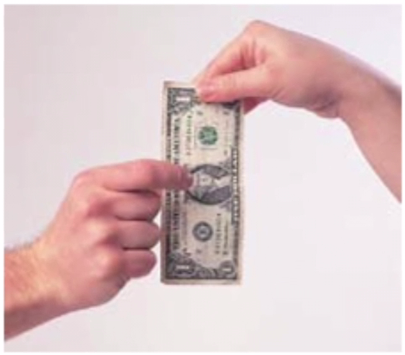
\includegraphics[width=.3\columnwidth]{imagenes/reto.png}
		\caption{Dibujo esquemático del reto entre Laura y Joel.}
		\label{fig:reto}
	\end{figure}

	\subsection{Ejercicio: Distancia Relativa \textcolor{red}{*}}
	Un globo desciende con velocidad constante de $10m/s$. En cierto momento su tripulante deja caer una piedra sin comunicarle ningún impulso. Halle la distancia entre el globo y la piedra en función del tiempo. Evalúela a los $5s$

	\textbf{Sugerencia:} Defina bien su marco de referencia y piense cual es la velocidad inicial de la piedra.

	\section{Movimiento 2D}

	\subsection{Ejercicio: Lanzamiento de un Proyectil}
	Se lanza desde el piso un proyectil con velocidad de $15m/s$ y un ángulo de $\psi$ con la horizontal.

	\begin{enumerate}[a)]
		\item Calcule el máximo alcance horizontal (R/ $22.96m$).
		\item Si hay una pared vertical de $18m$ del punto de lanzamiento, ¿con qué ángulo debe lanzarse la bala para golpear la pared lo mas alto posible y cuánto vale esa altura? En el momento en que la bola golpea la pared, ¿está subiendo o bajando? (R/ $51.90^{\circ}; 4.42m$)
		\item Si además de la pared vertical hay un techo horizontal a $4.5m$ sobre el piso, ¿cuál es ahora el punto más alto en el que puede golpearse la pared vertical con la bala y con qué ángulo debe lanzarse? (R/ $38.76^{\circ}; 2.85m$)
	\end{enumerate}

	\subsection{Ejercicio: Desastre en el Bar \textcolor{red}{*}}
	En un bar local, un cliente desliza sobre la barra un tarro de cerveza vacío para que lo vuelvan a llenar. El cantinero acaba de decidir ir a casa y repensar su vida, de modo que no ve el tarro. El tarro de desliza en la barra y golpea el suelo a una distancia $d$ de la base de la barra. La altura de la barra es $h$. a) ¿Con qué velocidad el tarro dejó la barra? b) ¿Cuál fue la dirección de la velocidad del tarro justo antes de golpear el suelo?

	\subsection{Ejercicio: Ligaduras}
	Dos objetos $A$ y $B$ se conectan mediante una barra rígida que tiene longitud $L$. Los objetos se deslizan a lo largo de rieles guía perpendiculares como se muestra en la (Fig. \ref{fig:ligaduras}). Suponga que $A$ se desliza hacia la derecha con una rapidez constante $v$. En encuentre la velocidad de $B$ en función de $\theta$ y cuando $\theta = 60^{\circ}$.\\

	\textbf{Nota:} Este tipo de acoples en las posiciones de los objetos se llaman \textit{ligaduras} y son muy comunes en la mecánica de cuerpos rígidos. En este caso, la ligadura es una barra rígida que conecta a los dos objetos. En general, las ligaduras pueden ser de diferentes tipos, como cuerdas, cadenas o barras, y pueden imponer diferentes restricciones de movimiento, velocidad y aceleración de los objetos.
	
	\begin{figure}[htbp]
		\centering
		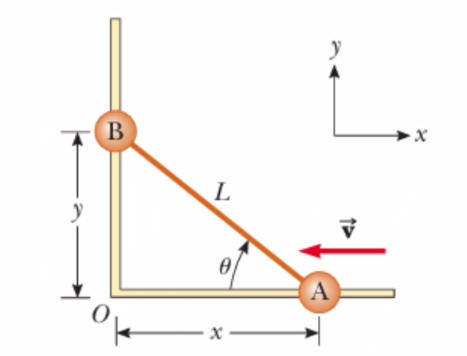
\includegraphics[width=.4\columnwidth]{imagenes/ligaduras.png}
		\caption{Dibujo esquemático de los objetos A y B.}
		\label{fig:ligaduras}
	\end{figure}

	\printbibliography[heading=bibintoc]
	
\end{document}